% Options for packages loaded elsewhere
\PassOptionsToPackage{unicode}{hyperref}
\PassOptionsToPackage{hyphens}{url}
%
\documentclass[
]{article}
\usepackage{lmodern}
\usepackage{amssymb,amsmath}
\usepackage{ifxetex,ifluatex}
\ifnum 0\ifxetex 1\fi\ifluatex 1\fi=0 % if pdftex
  \usepackage[T1]{fontenc}
  \usepackage[utf8]{inputenc}
  \usepackage{textcomp} % provide euro and other symbols
\else % if luatex or xetex
  \usepackage{unicode-math}
  \defaultfontfeatures{Scale=MatchLowercase}
  \defaultfontfeatures[\rmfamily]{Ligatures=TeX,Scale=1}
\fi
% Use upquote if available, for straight quotes in verbatim environments
\IfFileExists{upquote.sty}{\usepackage{upquote}}{}
\IfFileExists{microtype.sty}{% use microtype if available
  \usepackage[]{microtype}
  \UseMicrotypeSet[protrusion]{basicmath} % disable protrusion for tt fonts
}{}
\makeatletter
\@ifundefined{KOMAClassName}{% if non-KOMA class
  \IfFileExists{parskip.sty}{%
    \usepackage{parskip}
  }{% else
    \setlength{\parindent}{0pt}
    \setlength{\parskip}{6pt plus 2pt minus 1pt}}
}{% if KOMA class
  \KOMAoptions{parskip=half}}
\makeatother
\usepackage{xcolor}
\IfFileExists{xurl.sty}{\usepackage{xurl}}{} % add URL line breaks if available
\IfFileExists{bookmark.sty}{\usepackage{bookmark}}{\usepackage{hyperref}}
\hypersetup{
  pdftitle={TP1 Econometría Avanzada},
  pdfauthor={Casiano, Denys; Daboin, Carlos y Quispe, Anzony},
  hidelinks,
  pdfcreator={LaTeX via pandoc}}
\urlstyle{same} % disable monospaced font for URLs
\usepackage[left=2.5cm,right=2.5cm,top=1.5cm,bottom=2cm]{geometry}
\usepackage{graphicx,grffile}
\makeatletter
\def\maxwidth{\ifdim\Gin@nat@width>\linewidth\linewidth\else\Gin@nat@width\fi}
\def\maxheight{\ifdim\Gin@nat@height>\textheight\textheight\else\Gin@nat@height\fi}
\makeatother
% Scale images if necessary, so that they will not overflow the page
% margins by default, and it is still possible to overwrite the defaults
% using explicit options in \includegraphics[width, height, ...]{}
\setkeys{Gin}{width=\maxwidth,height=\maxheight,keepaspectratio}
% Set default figure placement to htbp
\makeatletter
\def\fps@figure{htbp}
\makeatother
\setlength{\emergencystretch}{3em} % prevent overfull lines
\providecommand{\tightlist}{%
  \setlength{\itemsep}{0pt}\setlength{\parskip}{0pt}}
\setcounter{secnumdepth}{-\maxdimen} % remove section numbering
\usepackage{booktabs} \usepackage{longtable} \usepackage{array} \usepackage{multirow} \usepackage{wrapfig} \usepackage{float} \usepackage{dcolumn} \floatplacement{figure}{H}

\title{TP1 Econometría Avanzada}
\author{Casiano, Denys; Daboin, Carlos y Quispe, Anzony}
\date{2022-04-11}

\begin{document}
\maketitle

\hypertarget{discusion-del-estimador-between}{%
\subsection{1. Discusion del estimador
between}\label{discusion-del-estimador-between}}

\emph{Discuta el modelo estimado (comente acerca de la validez del
estimador between y potenciales sesgos) y comente los resultados
obtenidos, en particular para las variables de justicia criminal.}

El modelo between al no considerar la heterogeneidad no observada del
condado produce estimadores similares a las estimaciones de corte
transversal. Esto genera un problema, ya que si las características no
observables están correlacionadas con \((X'_{it},P'_{it})\) se generarán
estimaciones sesgadas y por tanto inconsistentes. Dado el modelo con
transformación between presentado en el paper, esto significa que, el
estimador solo será consistente si \((X'_{it},P'_{it})\) son ortogonales
tanto a \(\alpha_i\) como a \(\epsilon_{it}\).

Los resultados del modelo muestran que las estimaciones para las
variables de justicia criminal (\(P_A, P_C, S\)) cumplen con el signo
negativo (sugerido por el modelo económico de crimen), a excepción de la
variable \(P_P\). Respecto de la significatividad estadística de las
estimaciones, solo los parámetros \(P_A\) y \(P_C\) son signficativos.
Es decir, según los resultados de este modelo, la probabilidad de
detención y la probabilidad de condena son significativas para explicar
la tasa de criminalidad. Finalmente, las estimaciones de los parámetros
en valor absoluto cumplen con el ordenamiento de los efectos disuasorios
del modelo de crimen donde \(P_A>P_C>P_P\).

\hypertarget{posibles-problemas-de-heterogeneidad-no-observable}{%
\subsection{2. Posibles problemas de heterogeneidad no
observable}\label{posibles-problemas-de-heterogeneidad-no-observable}}

\emph{Explique por qué es muy posible que la presencia de heterogeneidad
no observable a nivel de condado haga que las estimaciones anteriores
sean sesgadas. }

Dos condados pueden ser diferentes en \emph{confounders} no-observables
(confounders son variables correlacionadas con la variable dependiente y
las variables explicativas.)

Por ejemplo, es plausible que haya distintas tasas de reporte del crimen
entre distintos condados, lo cual es inchequeable ya que las denuncias
son la única manera de medir el crimen. De ser esto cierto, aquellos
condados similares a los demás en todas las características observables
pero con altas tasas de subreporte tendrán (en promedio) una menor tasa
de criminalidad y mayores tasas de arresto, lo que sesgaría la
estimación del efecto de las tasas de arresto sobre la criminalidad,
haciéndolo parecer de mayor magnitud.

\emph{Realice una estimación con efectos fijos por condado.}

\emph{Discuta por qué esta alternativa resolvería el problema de sesgo.
}\\
Un estimador de efectos fijos estaría exento de toda la variabilidad
atribuible a los condados, por lo que se esta controlando por todos los
factores no-observables que varían en este nivel.

Acerca del ejemplo anterior, un estimador de efectos fijos (también
llamado \emph{within}) hubiese corregido las bajas tasas de criminalidad
y las altas tasas de arresto de nuestros condados con alto subreporte,
haciéndolos comparables al resto.

\emph{Testee formalmente la hipótesis nula de ausencia de efectos fijos.
}

CD: Deberiamos comparar los estimadores del model between con los
estimadores del modelo de efecto fijo usando el test de Hausmann

\begin{gather*}
H = ( \hat \beta_{BE} - \hat \beta_{EF})' (\Omega_{EF}-\Omega_{BE})^{-1}  ( \hat \beta_{BE} - \hat \beta_{EF})
\end{gather*}

\begin{verbatim}
## 
##  Hausman Test
## 
## data:  lcrmrte ~ lprbarr + lprbconv + lprbpris + lavgsen + lpolpc +  ...
## chisq = 53.591, df = 16, p-value = 6.047e-06
## alternative hypothesis: one model is inconsistent
\end{verbatim}

El test de Hausman rechaza la hipótesis nula de ausencia de efectos
fijos, es decir, en base a este test se puede concluir que la
heterogeneidad es estadísticamente importante.

\emph{A la luz del trabajo de CyT, discuta las principales diferencias
encontradas con las estimaciones anteriores.}

El efecto de controlar por condado hace que las estimaciones (en valor
absoluto) de las variables de justicia disminuyan. Por ejemplo, para la
variable \(P_A\) la elasticidad estimada disminuyó aproximadamente
\(41\%\), mientras que para la variable \(P_C\) disminuyó \(43\%\)
aproximadamente. A diferencia de las estimaciones between, el
coeficiente \(P_P\) estimado por efectos fijos tiene no sólo el signo
correcto (negativo) sino es significativo estadísticamente. Al igual que
en el caso anterior, la estimación del parámetro \(S\) es no
significativa y de pequeño impacto. Finalmente, se pudo observar que los
efectos disuasorios estimador (en valor absoluto) se pueden ordenar
según el modelo económico del crimen (\(P_A>P_C>P_P\)).

\hypertarget{probando-el-estimador-de-efectos-aleatorios}{%
\section{3. Probando el estimador de efectos
aleatorios}\label{probando-el-estimador-de-efectos-aleatorios}}

Estime el modelo usando un estimador de efectos aleatorios. Implemente
un test de Hausman para comparar los estimadores de efectos fijos y de
efectos aleatorios y comente los resultados obtenidos

Al igual que en el caso anterior, el test de Hausman rechaza la
hipótesis nula de ausencia de efectos fijos, es decir, en base a este
test se puede concluir que la heterogeneidad es estadísticamente
importante. Esto se da debido a que las estimaciones por efectos
aleatorios no controlan efectos individuales, sino los trata como
variables omitidas generando sesgos si \((X'_{it},P'_{it})\) no son
ortogonales a \(\alpha_i\) y a \(\epsilon_{it}\).

\hypertarget{comparando-resultados}{%
\section{4. Comparando resultados}\label{comparando-resultados}}

\begin{table}[!htbp] \centering 
  \caption{Resultados} 
  \label{} 
\small 
\begin{tabular}{@{\extracolsep{5pt}}lD{.}{.}{-3} D{.}{.}{-3} D{.}{.}{-3} } 
\\[-1.8ex]\hline 
\hline \\[-1.8ex] 
 & \multicolumn{3}{c}{\textit{Dependent variable:}} \\ 
\cline{2-4} 
\\[-1.8ex] & \multicolumn{3}{c}{Tasa de criminalidad} \\ 
\\[-1.8ex] & \multicolumn{1}{c}{(1)} & \multicolumn{1}{c}{(2)} & \multicolumn{1}{c}{(3)}\\ 
\hline \\[-1.8ex] 
 $P_{A}$ & -0.648^{***} & -0.385^{***} & -0.415^{***} \\ 
  & (0.088) & (0.033) & (0.030) \\ 
  $P_{C}$ & -0.528^{***} & -0.301^{***} & -0.325^{***} \\ 
  & (0.067) & (0.021) & (0.020) \\ 
  $P_{P}$ & 0.297 & -0.191^{***} & -0.196^{***} \\ 
  & (0.231) & (0.033) & (0.033) \\ 
  S & -0.236 & 0.026 & 0.019 \\ 
  & (0.174) & (0.025) & (0.026) \\ 
  Police & 0.364^{***} & 0.424^{***} & 0.415^{***} \\ 
  & (0.060) & (0.027) & (0.025) \\ 
  Density & 0.168^{**} & 0.409 & 0.469^{***} \\ 
  & (0.077) & (0.279) & (0.051) \\ 
  Percent of young male & -0.095 & 0.381 & -0.132 \\ 
  & (0.158) & (0.325) & (0.123) \\ 
  WCON & 0.195 & -0.034 & -0.020 \\ 
  & (0.210) & (0.039) & (0.039) \\ 
  WTUC & -0.196 & 0.029^{*} & 0.025 \\ 
  & (0.170) & (0.018) & (0.018) \\ 
  WTRD & 0.129 & -0.039 & -0.035 \\ 
  & (0.278) & (0.041) & (0.042) \\ 
  WFIR & 0.113 & -0.013 & -0.017 \\ 
  & (0.220) & (0.029) & (0.029) \\ 
  WSER & -0.106 & 0.004 & -0.004 \\ 
  & (0.163) & (0.019) & (0.020) \\ 
  WMFG & -0.025 & -0.388^{***} & -0.264^{***} \\ 
  & (0.134) & (0.102) & (0.078) \\ 
  WFED & 0.156 & -0.553^{***} & -0.394^{***} \\ 
  & (0.287) & (0.165) & (0.144) \\ 
  WSTA & -0.284 & 0.216^{**} & 0.009 \\ 
  & (0.256) & (0.101) & (0.086) \\ 
  WLOC & 0.010 & 0.341^{***} & 0.209^{**} \\ 
  & (0.463) & (0.107) & (0.099) \\ 
  West & -0.230^{**} &  & -0.207^{**} \\ 
  & (0.108) &  & (0.105) \\ 
  Central & -0.164^{**} &  & -0.180^{***} \\ 
  & (0.064) &  & (0.062) \\ 
  Urban & -0.035 &  & -0.236^{**} \\ 
  & (0.132) &  & (0.114) \\ 
  Percent minority & 0.148^{***} &  & 0.199^{***} \\ 
  & (0.049) &  & (0.043) \\ 
  Constant & -2.097 &  & 0.252 \\ 
  & (2.822) &  & (0.561) \\ 
 \hline \\[-1.8ex] 
Observations & \multicolumn{1}{c}{90} & \multicolumn{1}{c}{630} & \multicolumn{1}{c}{630} \\ 
R$^{2}$ & \multicolumn{1}{c}{0.880} & \multicolumn{1}{c}{0.425} & \multicolumn{1}{c}{0.566} \\ 
Adjusted R$^{2}$ & \multicolumn{1}{c}{0.846} & \multicolumn{1}{c}{0.310} & \multicolumn{1}{c}{0.551} \\ 
F Statistic & \multicolumn{1}{c}{25.412$^{***}$ (df = 20; 69)} & \multicolumn{1}{c}{24.220$^{***}$ (df = 16; 524)} & \multicolumn{1}{c}{793.199$^{***}$} \\ 
\hline 
\hline \\[-1.8ex] 
\textit{Note:}  & \multicolumn{3}{l}{$^{*}$p$<$0.1; $^{**}$p$<$0.05; $^{***}$p$<$0.01} \\ 
\end{tabular} 
\end{table}

De la tabla de resultados se pudo observar que al igual que las
estimaciones por efectos fijos, las estimaciones por efectos aleatorios
de \(P_A\), \(P_C\) y \(P_P\) cumplen con los signos (negativos) y el
ordenamiento de los efectos disuasorios (excluyendo \(S\)) que afirma el
modelo económico de crimen (\(P_A>P_C>P_P\)). Respecto de la
significatividad estadística de las variables se pudo observar que en
ambas estimaciones los parámetros \(P_A\), \(P_C\) y \(P_P\) son
significativos.

Así también, se pudo observar que el no controlar por efectos del
condado genera sobrestimaciones en el primer y tercer modelo (between y
efectos aleatorios). Por ejemplo, para \(P_A\) la elasticidad se reduce
en un \(7.23\%\), mientras que para \(P_C\) lo hace en \(7.38\%\) y para
\(P_C\) en \(2.55\%\). Respecto de las diferencias entre la estimación
between y efectos fijos revisar el punto 2 del presente trabajo.

Al igual que en el modelo de efectos fijos, el signo del parámetro \(S\)
no coincide con lo estipulado en el modelo económico de crimen, es
pequeño y no es significativo a nivel estadístico.

Tal y como indican Cornwell y Trumbull, la no incorporación de efectos
por condado generan grandes diferencias en las estimaciones (en este
caso entre between, within y efectos aleatorios). Así también, dados los
test de Hausman se concluyó que la heterogeneidad es estadísticamente
importante en esta muestra y por lo tanto las estimaciones between y de
efectos aleatorios (quienes no incorporan esta característica en sus
estimaciones) deben ser rechazadas.

\hypertarget{comentarios-sobre-la-presencia-de-efectos-aleatorios-y-correlacion-serial-de-primer-orden}{%
\section{5. Comentarios sobre la presencia de efectos aleatorios y
correlacion serial de primer
orden}\label{comentarios-sobre-la-presencia-de-efectos-aleatorios-y-correlacion-serial-de-primer-orden}}

\hypertarget{including-plots}{%
\subsection{Including Plots}\label{including-plots}}

You can also embed plots, for example:

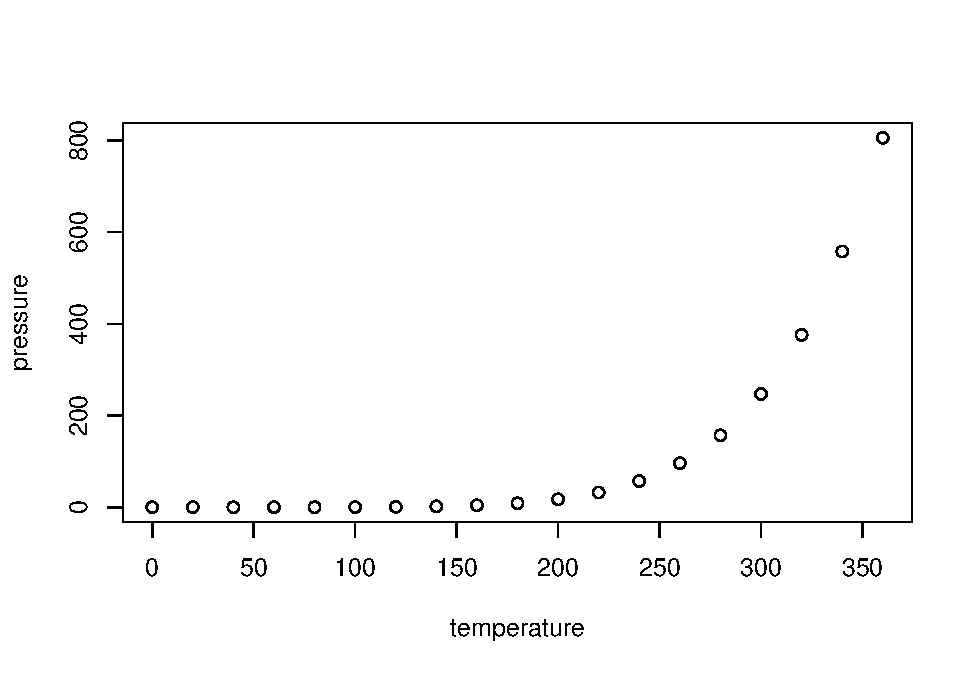
\includegraphics{TP2_Econometria_Avanzada_Casiano_Daboin_Quispe--1-_files/figure-latex/pressure-1.pdf}

Note that the \texttt{echo\ =\ FALSE} parameter was added to the code
chunk to prevent printing of the R code that generated the plot.

\end{document}
